\documentclass[a4paper, 11pt]{article}%тип документа
\usepackage{siunitx}
%отступы
\usepackage[left=2cm,right=2cm,top=2cm,bottom=3cm,bindingoffset=0cm]{geometry}
\usepackage[pdftex]{lscape}
%Русский язык
\usepackage[T2A]{fontenc} %кодировка
\usepackage[utf8]{inputenc} %кодировка исходного кода
\usepackage[english,russian]{babel} %локализация и переносы

%Вставка картинок
\usepackage{wrapfig}
\usepackage{graphicx}
\graphicspath{{Images/}}
\DeclareGraphicsExtensions{.pdf,.png,.jpg}

%Математика
\usepackage{amsmath, amsfonts, amssymb, amsthm, mathtools}

%Заголовокhttps://www.overleaf.com/project/6507f5a4176b25bf05722230
\author{Акимов М.И., Кондратюк Н.А. \\ Б06-206}

\title{Отчёт о выполнении лабораторной работы  \\ \textbf{pH - метрическое титрование аминокислот}}
\date{\\7 мая 2024 года}
\begin{document}
 \maketitle

       \section{Цели работы}
        \begin{itemize}
            \item Знакомство с потенциометрическими методами измерения рН растворов
            \item Приобретение практических навыков измерения рН
            \item Изучение ионного состава растворов аминоксилот при различных значениях рН
            \item Определение констант диссоциации выданной аминокислоты
        \end{itemize}

        \section{Задачи работы}
        \begin{itemize}
             \item Провести pH - метрическое титрование аминокислоты гистидин; 
             \item Определить константы диссоциации различных форм гистидина, построить экспериментальную и теоретическую кривые титрования, определить точки эквивалентности, построить теоретические зависимости концентраций различных форм гистидина в зависимости от pH и объёма титранта;
             \item Провести кондуктометрическое титрование гистидина;
             \item По экспериментальным данным оценить предельные удельные электропроводности ионов гистидина и гидроксид-ионов;
             \item Сделать выводы о соответствии полученных значений теоретическим.
        \end{itemize}
        \newpage
\section{Теоретическое введение}
\subsection{Устройство pH - метра}\;
\par При конструировании цепи для измерения рН необходимо обеспечить независимость потенциала электрода сравнения от состава исследуемого раствора. Например, для этого электроды объединяют в гальваническую ячейку, изображенную на Рис. 
\begin{wrapfigure}{l}{0.5\textwidth}
    \centering
    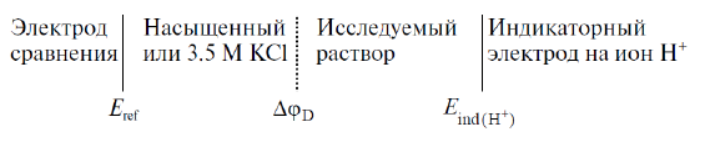
\includegraphics[width=0.5\textwidth]{Images/Снимок экрана 2024-05-07 125615.png}
    \caption{Гальваническая ячейка.}
\end{wrapfigure}\;
\par ЭДС представленной ячейки определяется следующим выражением:
\begin{equation*}
    E_x = E_{ind} - E_{ref} + \Delta \phi_D
    \eqno(1)
\end{equation*}
\par Индикаторный электрод на ион $H^+$ обычно представляет из себя стеклянный электрод с тонкой стеклянной мембраной. Уравнение, описывающее потенциал такого электрода была получено Б.П.Никольским:
\begin{equation*}
    E_{ind} = E_{ind}^0 + \frac{RT}{F}\ln{(a_{H^+} + Ka_{Na^+})}
    \eqno(2)
\end{equation*}
\par В кислых и нейтральных средах вклад протонов преобладает над катионным влиянием, а следовательно, уравнение (2) приобретает вид:
\begin{equation*}
    E_{ind} \approx E_{ind}^0 + \frac{RT}{F}\ln{(a_{H^+})}
    \eqno(3)
\end{equation*}
\par Потенциал сравнительного электрода легко считается по следующей формуле:
\begin{equation*}
    E_{ref} = E_{ref}^0 - \frac{RT}{F}\ln{(a_{Cl^-})}
    \eqno(4)
\end{equation*}
\par Подставляя в уравнение (1) полученные выражения, получим:
\begin{equation*}
    E_{x} = E_{ind}^0 + \frac{RT}{F}\ln{(a_{H^+})} - E_{ref}^0 + \frac{RT}{F}\ln{(a_{Cl^-})} + \Delta \phi_D
    \eqno(5)
\end{equation*}
\par Поскольку активность хлорид-ионов во внутреннем растворе электрода сравнения остаётся постоянной $a_{Cl^-} = const$, а диффузионный потенциал поддерживают на предельном нулевом значении, получаем следующее выражение для pH - метра:
\begin{equation*}
    E_{x} \approx E^0 - \frac{RT \ln{10}}{F} pH_x
    \eqno(6)
\end{equation*}
\subsection{pH - метрическое титрование аминокислот}\;
\par Аминокислоты в силу своей структуры имеют два и более химических центров, по которым может проводиться протонирование или депротонирование. От этого будет зависеть количество констант диссоциации гистидина по каждой из форм и форма кривой титрования. 
\begin{figure}
    \centering
    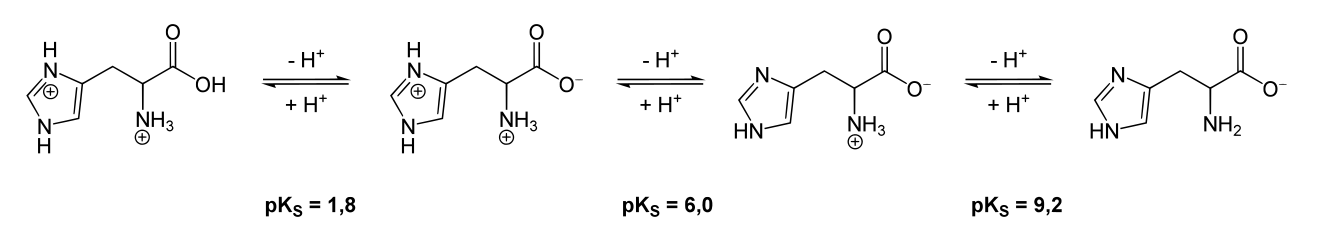
\includegraphics[width=0.7\textwidth]{Images/Гистидин.png}
    \caption{Формы гистидина.}
\end{figure}\;
\par Произведём теоретический рассчёт кривой титрования.
\par В растворе одновременно реализуются следующие равновесные реакции:

$$H_3A^{2+} \leftrightarrows H_2A^+ + H^+;\; K_1$$
$$H_2A^+ \leftrightarrows HA + H^+; \; K_2$$
$$HA \leftrightarrows A^- + H^+; \; K_3$$
$$H_2O \leftrightarrows OH^- + H^+; \; K_w$$
\par Они соответствуют следующим уравнениям:
\begin{equation*}
    K_1 = \frac{[H_2A^+][H^+]}{[H_3A^{2+}]}
    \eqno(7)
\end{equation*}
\begin{equation*}
    K_2 = \frac{[HA][H^+]}{[H_2A^+]}
    \eqno(8)
\end{equation*}
\begin{equation*}
    K_3 = \frac{[A^-][H^+]}{[HA]}
    \eqno(9)
\end{equation*}

\par Также для рассчёта можно использовать уравнение матбаланса и электронейтральности:
\begin{equation*}
    [A]_0 = [A^-] + [HA] + [H_2A^+] + [H_3A^{2+}]
    \eqno(10)
\end{equation*}
\begin{equation*}
     [A^-] + [Cl^-] + [OH^-] = [Na^+] + [H^+] + [H_2A^+] + 2[H_3A^{2+}]
    \eqno(11)
\end{equation*}
\par В итоге получаем выражения для концентраций каждой из форм гистидина:
\begin{equation*}
    [A^-] = \frac{[A]_0}{1 + \frac{[H^+]}{K_3} + \frac{[H^+]^2}{K_3K_2} + \frac{[H^+]^3}{K_3K_2K_1}}
    \eqno(12)
\end{equation*}
\begin{equation*}
    [HA] = \frac{[A^-][H^+]}{K_3}
    \eqno(13)
\end{equation*}
\begin{equation*}
   [H_2A^+] = \frac{[A^-][H^+]^2}{K_3K_2}
    \eqno(14)
\end{equation*}
\begin{equation*}
   [H_3A^{2+}] = \frac{[A^-][H^+]^3}{K_3K_2K_1}
    \eqno(15)
\end{equation*}
\par Тогда концентрация ионов натрия будет равна:
\begin{equation*}
   [Na^+] = \frac{C_tV_t}{V_t + V_0}
    \eqno(16)
\end{equation*}
\begin{equation*}
   [Na^+] = [A^-] + \frac{C_0V_0}{V_t + V_0} + \frac{K_w}{[H^+]} - [H^+] - \frac{[A^-][H^+]^2}{K_3K_2} - \frac{2[A^-][H^+]^3}{K_3K_2K_1}
    \eqno(17)
\end{equation*}
\section{Ход работы}
\subsection{pH - метрическое титрование}\;


\par В первой части экперимента проводят измерение зависимости рН раствора объема добавленной щёлочи и от объёма добавленной кислоты. $70$ мл $0,01$ М раствора аминокислоты разбавляют небольшими порциями $1$ М $KOH$ ($2$ М $HCl$) с помощью специальной пипетки и измеряют рН при каждом добавленном объёме соответствующего титранта. 

\par Построим экспериментальный график зависимости pH раствора гистидина от добавленного объёма. При этом объём добавленной щёлочи будем считать положительным, а кислоты - отрицательным. 

\par Также сравним полученную зависимость с теоретической. Для этого будем использовать уравнения (12), (16), (17). Кроме того, для расчёта будем использовать табличные значения констант диссоциации различных форм гистидина и начальные концентрации используемых растворов:
$$pK_{a1} = 1,70; \; pK_{a2} = 6,04; \; pK_{a3} = 9,09; \;$$
$$V_0 = 70 \; \text{мл}; \; [NaOH]_0 = 1 \; M;\; [HCl]_0 = 2 \; M;\; [His]_0 = 0,01\; M;\;$$

\par Нанесём обе зависимости на один график - Рис. 3. 
\begin{figure}[h!]
	\centering{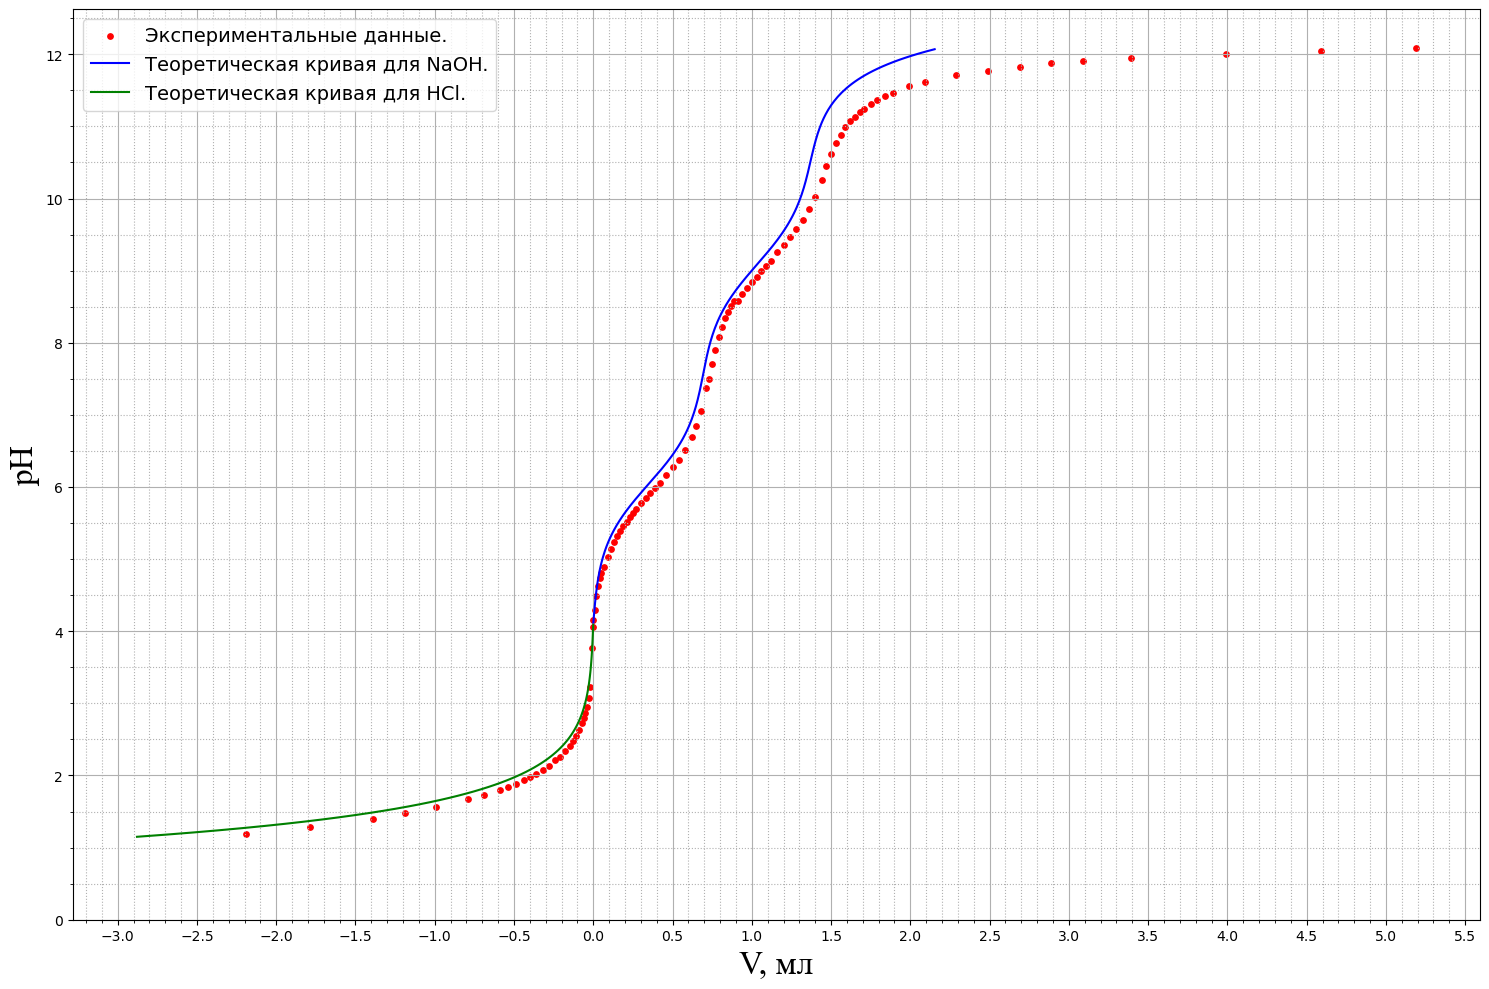
\includegraphics [scale=0.4]{Images/ТИТРЫ1.png}}
        \caption{Теоретическая и экспериментальная кривые титрования}
\end{figure}

\par Для экспериментального определения значений $pK_{a2}$ и $pK_{a3}$ построим график зависимости разностной производной $pH$ по $V$ от $pH$. Тогда локальные минимумы на графике будут соответствовать значениям констант кислотности. Рассчитанная зависимость представлена на Рис. 4. 


\par Определить значение $pK_{a1}$ экспеериментально не представляется возможным из-за недостатка данных. Экспериментальные значения двух других констант представлены ниже:
$$pK_{a2} = 5,91; \; pK_{a3} = 9,064;$$

\par Не будет лишним также найти значения точки эквивалентности. Сделать это можно по зависимости $\frac{\Delta pH}{\Delta V} (V)$ - максимумы на этом графике соответствуют точкам эквивалентности. Полученная кривая приведена на Рис. 5. 

\begin{figure}[h!]
	\centering{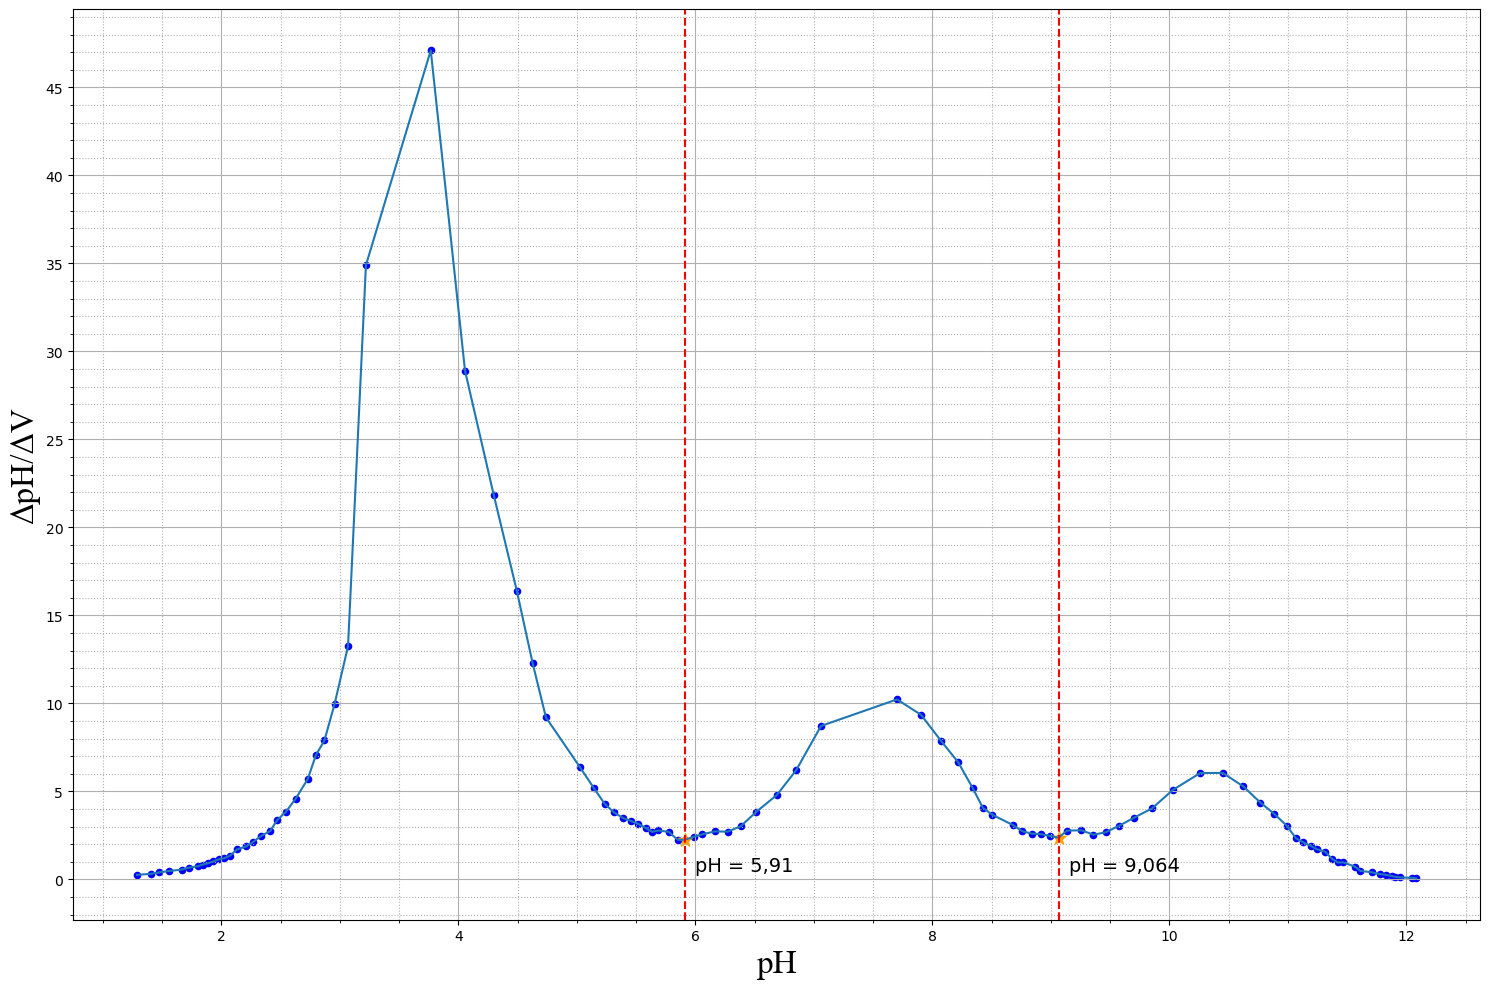
\includegraphics [scale=0.4]{Images/ТИТРЫ2.png}}
        \caption{График зависимости $\frac{\Delta pH}{\Delta V} (pH)$}
\end{figure}
\begin{figure}[h!]
	\centering{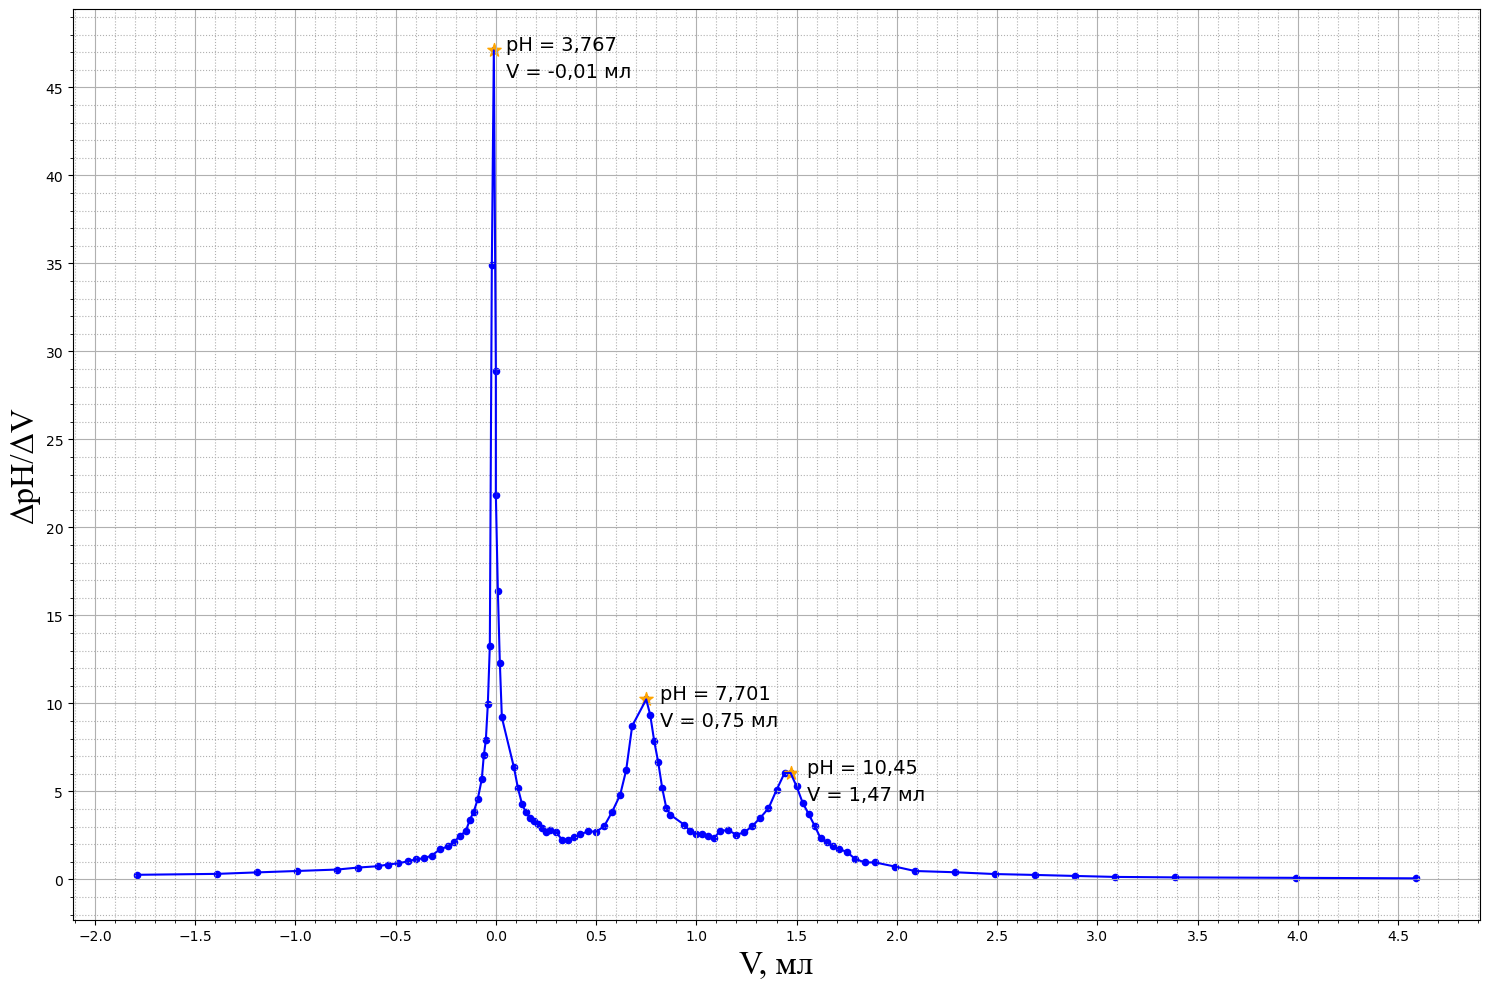
\includegraphics [scale=0.4]{Images/ТИТРЫ3.png}}
        \caption{График зависимости $\frac{\Delta pH}{\Delta V} (V)$}
\end{figure}
\par Полученные значения точек эквивалентности соответственно равны:


$$pH = 3,767, \; V = -0,01 \; \text{мл} \; (0,01 \; \text{мл} \; HCl)$$
$$pH = 7,701, \; V = 0,75 \; \text{мл}$$
$$pH = 10,45, \; V = 1,47 \; \text{мл}$$

\par Основываясь также на формулах (12), (13), (14), (15) построим графики зависимоcти $C(pH)$ и $C(V)$ - Рис. 6 и Рис. 7.
\newpage


 \begin{figure}[!htb] 
        \minipage{0.5\textwidth}
            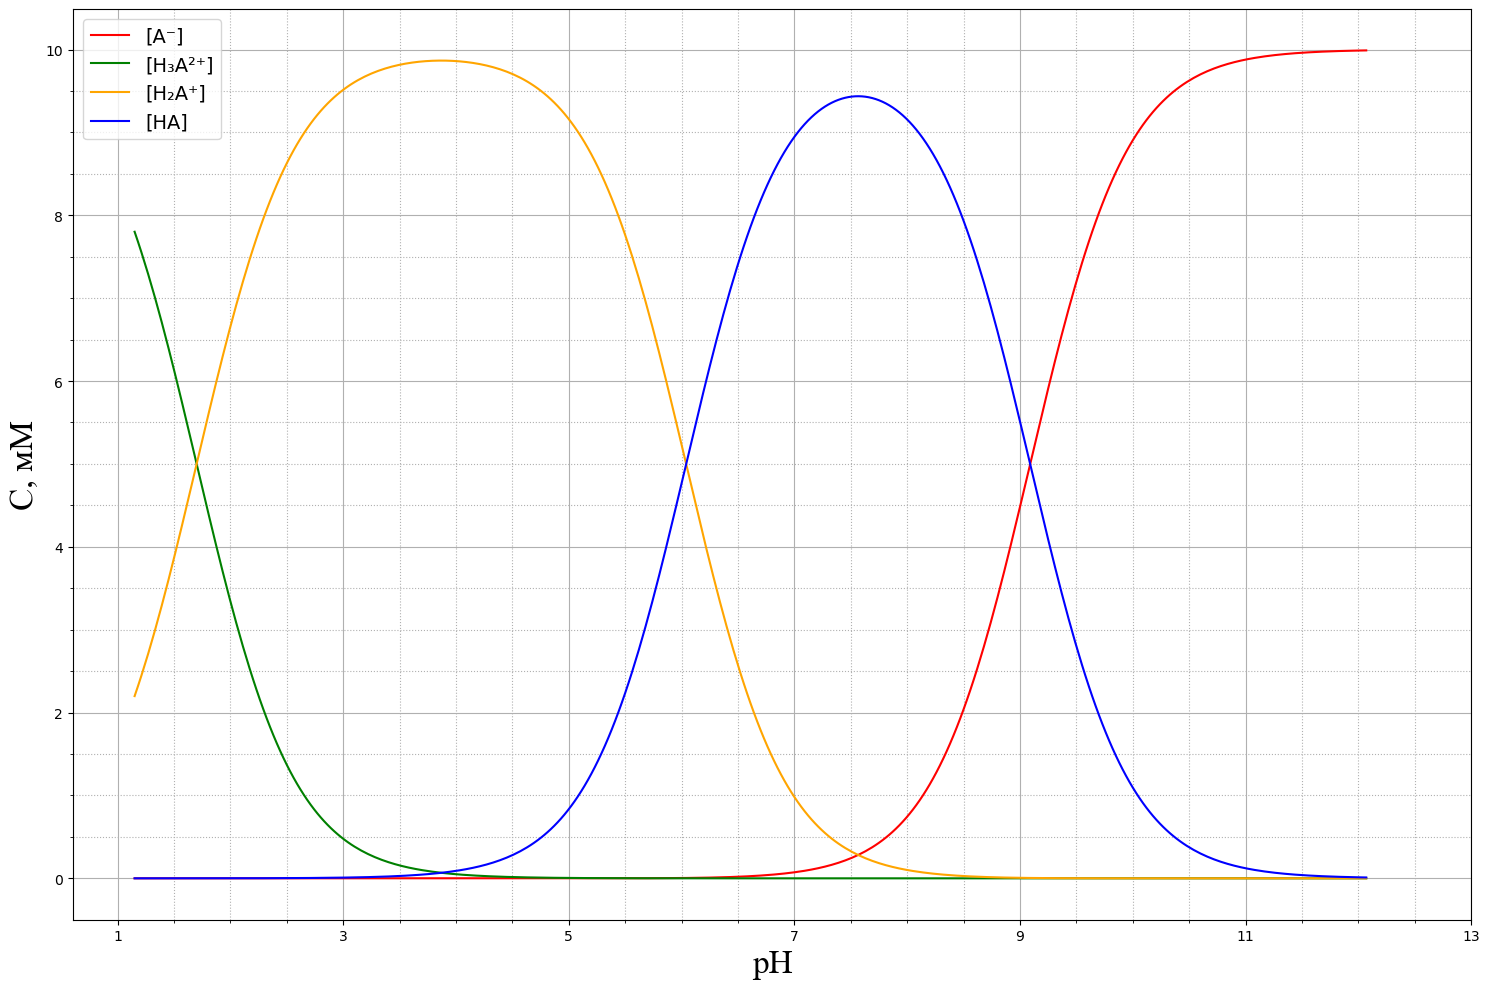
\includegraphics[width=\linewidth]{Images/ТИТРЫ4.png}
            \caption{Графики зависимости $C(pH)$}
        \endminipage\hfill
        \minipage{0.5\textwidth}
             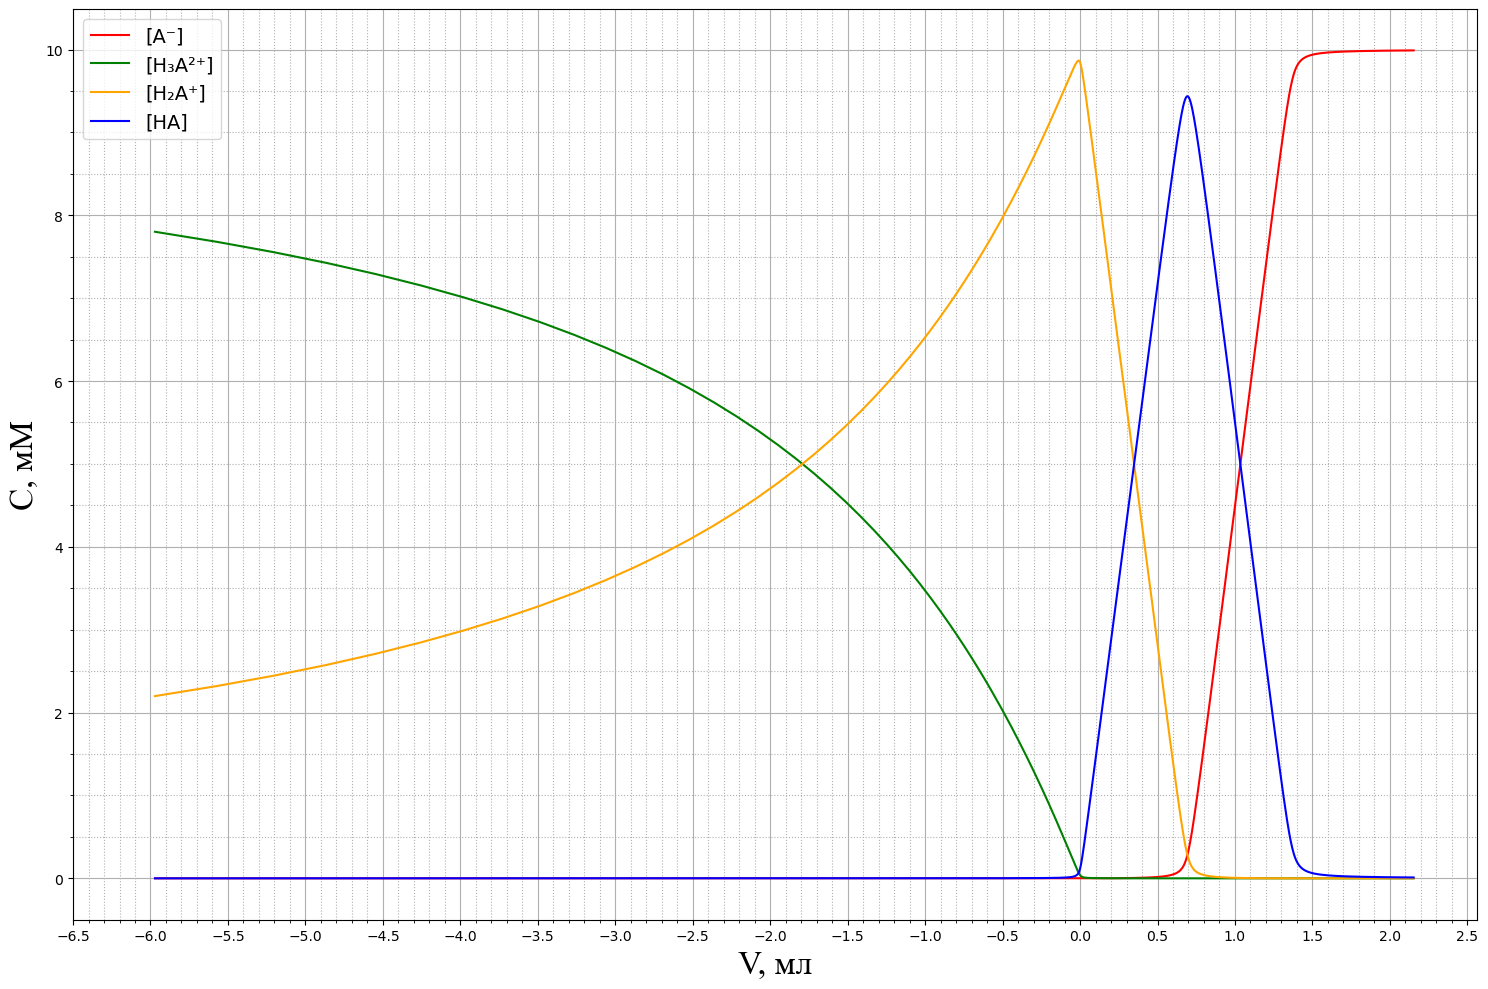
\includegraphics[width=\linewidth]{Images/ТИТРЫ6.png}
              \caption{Графики зависимости $C(V)$}
        \endminipage
    \end{figure}

\subsection{Кондуктометрическое титрование}
    \par Исследуем зависимость удельной электропроводности раствора аминокислоты гистидина от объёма добавленной щёлочи/кислоты при титровании. Для этого построим экспериментальный график (Рис. 8), где отрицательным значениям по оси абсцисс будет соответствовать добавление кислоты, а положительным - щёлочи. А также, рассмотрим последний участок кривой кондуктометрического титрования подробнее (Рис.9). 
    \begin{figure}[!htb] 
        \minipage{0.5\textwidth}
            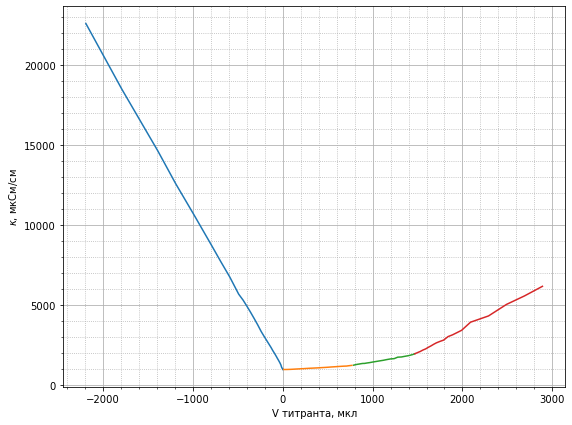
\includegraphics[width=\linewidth]{Images/тильт1.png}
            \caption{График зависимости $\kappa (\text{V титранта})$}
        \endminipage\hfill
        \minipage{0.5\textwidth}
             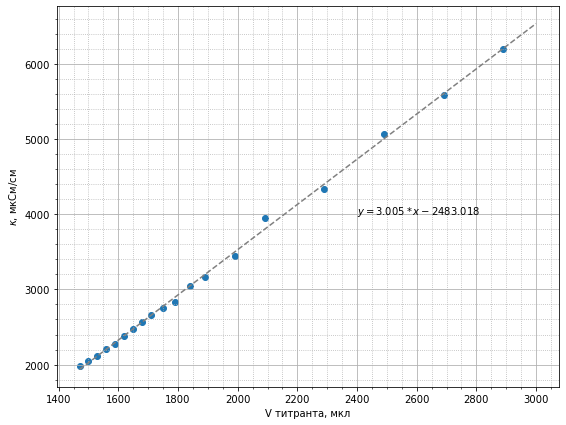
\includegraphics[width=\linewidth]{Images/тильт2.png}
              \caption{График зависимости $\kappa (\text{V титранта})$}
        \endminipage
    \end{figure}
    \par Проводимость на конечном участке определяется следующим выражением:
    \[\varkappa = \lambda_{Na^+}[Na^+] + \lambda_{OH^-}[OH^-] + \lambda_{Cl^-}[Cl^-] + \lambda_{A^-}[A^-]\]
    \par При таком избыточном добавлении щёлочи будем считать верным следующее выражение:
    \[ [A]_0 = [A^-] = [Cl^-]\]
    \par Распишем условие электронейтральности:
    \[ [Na^+] = [A^{-}]+[OH^{-}]+[Cl^{-}] \Rightarrow [OH^{-}]=[Na^{+}]-2[A]_{0}\]
    \[ [Na^{+}]=\frac{[Na^{+}]_{0}V}{V_0+V}\approx \frac{[Na^{+}]_{0}V}{V_0} \]
    \par Итого получаем:
    
    \[ \varkappa = \frac{[Na^{+}]_{0}V}{V_0} \cdot (\lambda_{Na^+} + \lambda_{OH^-}) + [A]_0 \cdot (\lambda_{Cl^-} + \lambda_{A^-} - 2\lambda_{OH^-})\]
    \[ \alpha =  \frac{[Na^{+}]_{0}}{V_0} \cdot (\lambda_{Na^+} + \lambda_{OH^-}) \]

    
    \par Конечная формула, которую будем использовать для расчёта эквивалентной электроповодности $OH^-$, представлена ниже:
    \[\lambda_{0}(OH^{-})=\frac{\alpha V_0}{[Na^{+}]_{0}}-\lambda_{0}(Na^{+})\]
    \par Из табличных данных:
    \[\lambda_{0}(Na^{+})=50,3 \frac{\text{См}\cdot\text{см}^{2}}{\text{моль}}\]
    \par Из угла наклона графика получаем:
    
    \[\alpha=3,005\frac{\text{мкСм}}{\text{мкл}\cdot\text{см}}=3,005\frac{\text{См}}{\text{л}\cdot\text{см}}\]

    \[\alpha V_{0} = 3,005\frac{\text{См}}{\text{л}\cdot\text{см}} \cdot 70 \cdot 10^{-3} \text{л}=210,35\cdot 10^{-3}\frac{\text{См}}{\text{см}}\]

    \[\frac{\alpha V_{0}}{[Na^{+}]_{0}} =\frac{210,35\cdot 10^{-3}\frac{\text{См}}{\text{см}}}{1\frac{\text{моль}}{\text{л}}}=210,35\frac{\text{См}\cdot\text{см}^{2}}{\text{моль}}\]

    \[\lambda_{0}(OH^{-})=\frac{\alpha V_0}{[Na^{+}]_{0}}-\lambda_{0}(Na^{+})=210,35-50,3=160,05\frac{\text{См}\cdot\text{см}^{2}}{\text{моль}}\]
    \[\lambda_{0}(A^{-})= 73,398\frac{\text{См}\cdot\text{см}^{2}}{\text{моль}}\]
    \par Такие же рассуждения мы можем провести для каждого из оставшихся трёх участков и определить значения удельных проводимостей для каждой из форм аминокислоты (Таблица 1). 

    \begin{table}[h!]
    \centering
    \begin{tabular}{|l|l|l|}
    \hline
    Участок & Коэффициент наклона k & Свободный член b \\ \hline
    1       & -9.765                & 1054.730         \\ \hline
    2       & 0.333                 & 975.637          \\ \hline
    3       & 0.988                 & 480.171          \\ \hline
    4       & 3.005                 & -2483.018        \\ \hline
    \end{tabular}
    \caption{Значения коэффициентов для каждого из участков графика кондуктометрического титрования}
    \end{table}
    \par Для простоты подсчёта можно исследовать систему в точках эквивалентности:
    \par \textbf{Участок 3} Рассмотрим точку эквивалентности $[A^{-}]=[HA]= \frac{C_{0}}{2}=0,005 \text{M}$ при $pH = 10,45 \; V = 1,47 \; \text{мл} \Rightarrow \varkappa = 1978 \frac{\text{мкСм}}{\text{см}}$. $[OH^{-}]= 10^{-pOH}=10^{10,45-14}=2,81 \cdot 10^{-4} M$. Электропроводность определяется аналогично
    \[\varkappa = \lambda_{Na^+}[Na^+] + \lambda_{OH^-}[OH^-] + \lambda_{Cl^-}[Cl^-] + \lambda_{A^-}[A^-]\]
    \par Подставляя значения, получаем $\lambda_{0}(A^{-})= 24,901 \frac{\text{См}\cdot\text{см}^{2}}{\text{моль}}$
    \par \textbf{Участок 2} Рассмотрим точку эквивалентности $[H_{2}A^{+}]=[HA]= \frac{C_{0}}{2}=0,005 \text{M}$ при $pH = 7,701 \; V = 0,75 \; \text{мл} \Rightarrow \varkappa = 1239 \frac{\text{мкСм}}{\text{см}}$. $[OH^{-}]= 10^{-pOH}=10^{7,701-14}=5,023 \cdot 10^{-7} M$. Электропроводность определяется
    \[\varkappa = \lambda_{Na^+}[Na^+] + \lambda_{OH^-}[OH^-] + \lambda_{Cl^-}[Cl^-] + \lambda_{H_{2}A^{+}}[H_{2}A^{+}]\]
    \par Подставляя значения, получаем $\lambda_{0}(H_{2}A^{+})= 11,46\frac{\text{См}\cdot\text{см}^{2}}{\text{моль}}$
    \par \textbf{Участок 1} Рассмотрим точку эквивалентности $[H_{2}A^{+}]=[H_{3}A^{2+}]= \frac{C_{0}}{2}=0,005 \text{M}$ при $pH = 3,77 \; V = -0,01 \; \text{мл} \Rightarrow \varkappa = 1093 \frac{\text{мкСм}}{\text{см}}$. $[H^{+}]= 10^{-pH}=10^{-3,77}=1,69 \cdot 10^{-4} M$. Электропроводность определяется
    \[\varkappa =  \lambda_{H^+}[H^+] + \lambda_{Cl^-}[Cl^-] + \lambda_{H_{2}A^{+}}[H_{2}A^{+}] + 2\lambda_{H_{3}A^{2+}}[H_{3}A^{2+}]\]
    \par Подставляя значения, получаем $\lambda_{0}(H_{3}A^{2+})= 19,175\frac{\text{См}\cdot\text{см}^{2}}{\text{моль}}$
    \section{Выводы}
    \begin{itemize}
        \item По экспериментальным данным, полученным в ходе pH - метрического титрования, была получена экспериментальная кривая титрования. На основе зависимости разностной производной от pH растворе были выведены следующие константы диссоциации форм гистидина:
        $$pK_{a2} = 5,91; \; pK_{a3} = 9,064;$$
        \item Также в ходе обработки результатов были найдены точки эквивалентности:
        $$pH = 3,767, \; V = -0,01 \; \text{мл} \; (0,01 \; \text{мл} \; HCl)$$
        $$pH = 7,701, \; V = 0,75 \; \text{мл}$$
        $$pH = 10,45, \; V = 1,47 \; \text{мл}$$
 
        \item Было исследовано изменение удельной проводимости раствора гистидина при титровании щёлочью и кислотой. Из полученных значений были экспериментально определены следующие предельные эквивалентные проводности:
        \begin{table}[h!]
    \centering
    \begin{tabular}{|l|l|}
    \hline
    Частица & Экв. проводность, $\frac{\text{См}\cdot\text{см}^{2}}{\text{моль}}$ \\ \hline
    $\lambda_{0}(OH^{-})$    & 160,05                \\ \hline
    $\lambda_{0}(A^{-})$    & 73,398                \\ \hline
    $\lambda_{0}(H_{2}A^{+})$    & 11,46                 \\ \hline
    $\lambda_{0}(H_{3}A^{2+})$    & 19,175                \\ \hline
\end{tabular}
\caption{Результаты анализа кондуктометрической кривой титрования}
\label{tab:my-table}
\end{table}
    \end{itemize}
\end{document}
